%\documentclass[notheorems]{beamer}
%\documentclass[handout]{beamer}
%\documentclass[handout,notes=show]{beamer}

\usetheme{metropolis}
%\usecolortheme{dolphin}
% No navigation bars
\beamertemplatenavigationsymbolsempty
\setbeamertemplate{footline}{}


\usepackage{amsmath, amssymb, amsfonts, tikz}
\usepackage[utf8]{inputenc}
\usepackage[T1]{fontenc}
\usepackage[english]{babel}
\usepackage{tabularx}
\usepackage{mathtools}
\usepackage{xmpmulti}
\usepackage{wrapfig}
\usepackage{listings}

\makeatletter
\let\@@magyar@captionfix\relax
\makeatother
\usepackage{floatrow}
\usepackage{caption}

\definecolor{identifiers}{rgb}{0.375,0,0.375}
\definecolor{comments}{rgb}{0.5,0,0}
\definecolor{strings}{rgb}{0,0.5,0}
\definecolor{keywords}{rgb}{0,0,0.5}
%% We define a null language, free of any formatting or style
%% for use when a language is not supported, or pseudo-code
\lstdefinelanguage{none}{identifierstyle=,commentstyle=,stringstyle=,keywordstyle=}
%% A style, both text behavior and decorations all at once
\lstdefinestyle{programstyle}{breaklines=true,breakatwhitespace=true,columns=fixed,frame=leftline,framesep=3ex, xleftmargin=3ex,
basicstyle=\small\ttfamily,identifierstyle=\color{identifiers},commentstyle=\color{comments},stringstyle=\color{strings},keywordstyle=\color{keywords}}
%% The environments manufactured by the listings package
%% Two environments, one full-width, the other boxed for side-by-sides
%% "program" expects a language argument only
%% "programbox" expects a language and a linewidth
\newenvironment{listing}{\par\bigskip\noindent}{}
\lstnewenvironment{program}[1][]
  {\lstset{style=programstyle,#1}}
  {}
\lstnewenvironment{programbox}[1][]
  {\lstset{style=programstyle,#1}}
  {}


\lstdefinelanguage{Sage}[]{Python}
{morekeywords={True,False,sage,singular},
sensitive=true}
\lstset{frame=none,
          showtabs=False,
          showspaces=False,
          showstringspaces=False,
          commentstyle={\ttfamily\color{dredcolor}},
          keywordstyle={\ttfamily\color{dbluecolor}\bfseries},
          stringstyle ={\ttfamily\color{dgraycolor}\bfseries},
          language = Sage,
      basicstyle={\small \ttfamily},
      aboveskip=.3em,
      belowskip=.1em
          }
\definecolor{dblackcolor}{rgb}{0.0,0.0,0.0}
\definecolor{dbluecolor}{rgb}{.01,.02,0.7}
\definecolor{dredcolor}{rgb}{0.8,0,0}
\definecolor{dgraycolor}{rgb}{0.30,0.3,0.30}
\newcommand{\dblue}{\color{dbluecolor}\bf}
\newcommand{\dred}{\color{dredcolor}\bf}
\newcommand{\dblack}{\color{dblackcolor}\bf}

\renewcommand{\emph}[1]{{\dblack{#1}}}

\newcommand{\Sage}{{\color{dbluecolor}\sf Sage}\xspace}




\setsansfont[
    Extension      = .otf,
    UprightFont    = *-Light,
    ItalicFont     = *-LightItalic,
    BoldFont       = *-Regular,
    BoldItalicFont = *-RegularItalic
]{FiraSans}
\setmonofont[
    Extension   = .otf,
    UprightFont = *-Regular,
    BoldFont    = *-Medium
]{FiraMono}

\definecolor{Purple}{HTML}{911146}
\definecolor{Orange}{HTML}{CF4A30}
\definecolor{Tan}{RGB}{225,221,191}
\definecolor{Green}{RGB}{76,131,122}
\definecolor{DB}{RGB}{4,37,58}

% Theme colors are derived from these two elements
\setbeamercolor{alerted text}{fg=Green}

% ... however you can of course override styles of all elements
\setbeamercolor{frametitle}{bg=Tan,fg=DB}

\metroset{titleformat=smallcaps}


\newcommand{\downleadsto}{\rotatebox[origin=c]{-90}{$\leadsto$}}
\usepackage{amsthm}
\theoremstyle{plain}
\newtheorem{theorem}{Theorem}[section]
\newtheorem{corollary}[theorem]{Corollary}
\newtheorem{lemma}[theorem]{Lemma}
\newtheorem{algorithm}[theorem]{Algorithm}
\newtheorem{proposition}[theorem]{Proposition}
\newtheorem{claim}[theorem]{Claim}
\newtheorem{fact}[theorem]{Fact}
\newtheorem{conjecture}[theorem]{Conjecture}
%% Definition-like environments, normal text
%% Numbering is in sync with theorems, etc
\theoremstyle{definition}
\newtheorem{definition}[theorem]{Definition}
%% Remark-like environments, normal text
%% Numbering is in sync with theorems, etc
\theoremstyle{definition}
\newtheorem{remark}[theorem]{Remark}
\newtheorem{observation}[theorem]{Observation}
%% Example-like environments, normal text
%% Numbering is in sync with theorems, etc
\theoremstyle{definition}
\newtheorem{example}[theorem]{Example}
\newtheorem{question}[theorem]{Question}
\newcommand{\terminology}[1]{\textbf{#1}}

\newcommand{\NN}{\mathbf{N}}
\newcommand{\ZZ}{\mathbf{Z}}
\newcommand{\QQ}{\mathbf Q}
\newcommand{\CC}{\mathbf C}
\newcommand{\RR}{\mathbf R}
\newcommand{\FF}{\mathbf F}
\newcommand{\lt}{<}
\newcommand{\gt}{>}
\newcommand{\amp}{&}
\newcommand{\diff}{\mathop{}\!\mathrm{d}}
\newcommand{\ints}{\mathcal{O}}
\newcommand{\ideal}[1]{\mathfrak{#1}}
\usepackage{mathrsfs}\usepackage{cancel}
\newcommand{\Gal}[2]{\operatorname{Gal}(#1/#2)}
\newcommand{\absgal}[1]{\operatorname{Gal}(\overline{#1}/#1)}
\DeclareMathOperator{\USp}{USp}
\DeclareMathOperator{\Spec}{Spec}

\DeclareMathOperator{\rank}{rank}
\newcommand{\sheaf}[1]{\operatorname{\mathcal{#1}}}
\DeclareMathOperator{\Jac}{Jac}
\newcommand{\inv}{^{-1}}
\DeclareMathOperator{\norm}{Nm}
\DeclareMathOperator{\ord}{ord}
\DeclareMathOperator{\divisor}{div}
\DeclareMathOperator{\PP}{\mathbf{P}}
\DeclareMathOperator{\Hom}{Hom}
\DeclareMathOperator{\Mat}{Mat}
\DeclareMathOperator{\End}{End}

\newcommand{\lb}{[}
\newcommand{\rb}{]}

\setbeamerfont*{subtitle}{size=\small,shape=\scshape}

\author{Alex J. Best}
\institute{Boston University}
\date{27/6/2019}
\title{Explicit computation with Coleman integrals}
\subtitle{BU -- Keio Workshop 2019}

\begin{document}

\begin{frame}
  \titlepage

  \note[item]{Thank the audience for being awake.}
\end{frame}

%\begin{frame}
%\frametitle{Table of Contents}
%\tableofcontents[currentsection]
%\end{frame}

\begin{frame}{Why do we integrate things? Logarithms}
    \note{there are many answers to this question}
    Take \( \frac{\diff x}{x}\), as a differential on the group \( \RR^\times \), \pause
    this is translation invariant, i.e. $(a\cdot - )^*(\diff x/x)= \diff(ax)/ax = \diff x/ x$\pause, hence
    \[
        \int_1^t \frac{\diff x}x = \log |t| \colon \RR^\times \to \RR
    \]
    has the property that
    \[
        \int_1^{ab} \frac{\diff x}x = \int_a^{ab} \frac{\diff x}{x} + \int_1^a \frac{\diff x}{x} = \int_1^b \frac{\diff x}{x}  + \int_1^a \frac{\diff x}{x}
    \]

    Integration can define logarithm maps between groups and their tangent spaces.

    How do we calculate $\log |t|$? Power series on $\RR_{\gt 0}$ and use the relation $\log|t| = \frac 12 \log t^2$

\end{frame}

\begin{frame}{Why do we integrate things? Interesting functions}

    We have already seen \emph{polylogarithms}, defined recursively by%#[m L_k
    \[
        L_1(z) = -\log(1-z),\,L_k(z)  = \int_0^z L_{k-1}(s)\frac{\diff s}{s} \colon \CC\smallsetminus [1,\infty) \to \CC
    \]\pause
    These functions can alternatively be described via the power series
    \[
        L_k(z) = \sum_{n=1}^\infty \frac{z^n}{n^k}
    \]

\end{frame}

\begin{frame}{Coleman integration}
    \note{As number theorists it is natural to ask,}
    Is there $p$-adic analogue of this?\visible<2->{
    Given a $p$-adic space, (as $p$-adic solutions to some equations) we can locally write down convergent power series for a 1-form and integrate.}


\begin{wrapfigure}{r}{0.45\textwidth}
\visible<5->
{
    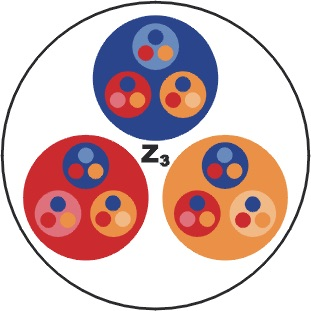
\includegraphics[width=0.45\textwidth]{padic.jpg}
}
\caption*{\visible<5->{Bad topology!}}
\end{wrapfigure}

\visible<3->{
    E.g. near a point $\alpha $:
\[\omega=\frac{\mathrm{d}(\alpha+x)}{\alpha+x}=\frac{\mathrm{d} x}{\alpha+x}=\frac{1}{\alpha} \sum\left(\frac{-x}{\alpha}\right)^{n} \mathrm{d} x\]}


\visible<4->{
    so that
\[\int_{\alpha + x}\omega = -\sum \frac{1}{n+1}\left(\frac{-x}{\alpha}\right)^{n+1}+C\]}

\visible<5->
{
    But we cannot find $C$! There is a different choice in each disk.
}

\end{frame}

\begin{frame}{Coleman integration: More problems}
    Now we have functions
    \[\mathrm{T}=\mathrm{K}\left\langle t\right\rangle=\left\{\sum a_{\mathrm{i}} t^{\mathrm{i}} ; a_{\mathrm{i}} \in \mathrm{K}, \lim _{\mathrm{i} \rightarrow \infty}\left|a_{\mathrm{i}}\right|=0\right\}\]
    and
    \[\diff \colon T \to \Omega ^1_{T}\]
    and our integral map should send
    \[ \sum a_{i} t^{i+1}\mapsto\sum \frac{a_{i}}{i+1} t^{i+1} \]
    but
    \[\frac{a_i}{i+1}\]
    may not converge to 0.

    So instead we work with a subring of \emph{overconvergent} functions
    \[\mathcal{T}^{\dagger}=\left\{\sum a_{\mathrm{i}} t^{\mathrm{i}} ; a_{\mathrm{i}} \in K, \exists r>1 \text { such that } \lim _{\mathrm{i} \rightarrow \infty}\left|a_{\mathrm{i}}\right| r^{\mathrm{i}}=0\right\}\text.\]

\end{frame}


\begin{frame}{Coleman's theorem}
    Take \(X/\ZZ_p\) a genus \(g\) curve, and \(p\) an odd prime.

    We pick a lift of the Frobenius map, i.e. \(\phi\colon X \to X\) which reduces to the Frobenius on $X\times \FF_p$, and write \(A^\dagger\) (resp.\ \(A_{\text{loc}}(X)\)) for overconvergent (resp.\ locally analytic) functions on \(X\).
    \pause%
    \begin{theorem}[{Coleman}]\label{thm-coleman-harvey-int}
        There is a \(\QQ_p\)-linear map \(\int_b^x\colon \Omega_{A^\dagger}^1\otimes \QQ_p \to A_\mathrm{loc} (X)\) for which:\leavevmode%
        \[\diff \circ \int_b^x = \mathrm{id}\colon \Omega_{A^\dagger}^1\otimes \QQ_p \to \Omega_{\text{loc}}^1\,\quad\text{``FTC''}\]%
        \[\int_b^x\circ\diff = \mathrm{id}\colon A^\dagger \hookrightarrow A_{\mathrm{loc}}\]%
        \[\int_b^x \phi^*\omega = \phi^*\int_b^x \omega\,\quad\text{``Frobenius equivariance''}\]%
    \end{theorem}

    This also works over extensions of $\QQ_p$.

\end{frame}

\begin{frame}{Computation: Polylogarithms on $\PP^1\smallsetminus \{0,1,\infty \}$}
    Let's revisit the \emph{polylogarithms}
    \[
        L_1(z) = -\log(1-z),\,L_k(z)  = \int_0^z L_{k-1}(s)\frac{\diff s}{s} \colon \CC\smallsetminus [1,\infty) \to \CC
    \]

    Coleman integration then defines a $p$-adic analogue of these functions, with exactly the same definition via iterated integration on $\PP^1\smallsetminus\{0,1,\infty\}$.

    (We must choose a branch of the $p$-adic logarithm, for simplicity we take the \emph{Iwasawa logarithm} where $\log_p(p)= 0$.)

    The power series definition still holds near $z=  0$, but otherwise we must use frobenius equivariance to define it.

\end{frame}

\begin{frame}[fragile]{Computing polylogarithms}

    Besser and de Jeu have given a complete algorithm to compute these functions, and this is now implemented in SageMath.

    For instance in Sage we can check relations among polylogarithms
\begin{programbox}[language=Sage]
sage: K = Qp(7, prec=30)
sage: x = K(1/3)
sage: (x^2).polylog(4) - 8*x.polylog(4) - 8*(-x).polylog(4)
O(7^23)
\end{programbox}\pause
In exactly the same way as:
\begin{programbox}[language=Sage]
sage: x = RBF(1/3) # Real ball, or do pari(1/3)
sage: (x^2).polylog(4) - 8*x.polylog(4) - 8*(-x).polylog(4)
[+/- 2.51e-14]
\end{programbox}


\end{frame}

\begin{frame}{Computation: group structure}
    If $X/\QQ_p$ is an algebraic group, $\omega $ is a translation invariant 1-form we have

    \[\int_0^{P+Q} \omega  = \int_0^P \omega + \int_0^Q \omega \implies \int_0^{P} \omega  = \frac 1n\int_0^{nP} \omega \]

    but if $n = \# \tilde X(\FF_p)$ then $nP \in B(0,1)$ so the integral on the right can be performed locally with only power series.

    \pause
    This requires arithmetic in the group, which may be hard.
    And can only integrate invariant differentials.


\end{frame}

\begin{frame}{Computation: $p$-adic cohomology}
    There is an alternate approach via $p$-adic cohomology, due to Balakrishnan-Bradshaw-Kedlaya.

    Let $X/\ZZ_p$ be a smooth curve of good reduction.

    Pick a basis $\omega_1, \ldots, \omega_{2g}$ for $H^1_\mathrm{dR}(X)$ and let $U \subseteq X$ be an affine subspace containing no poles of any $\omega_i$ and on which we have a lift of frobenius $\phi$.\pause

    If we apply $\phi^*$ to $\omega_i$ we may write
    \[\phi^* \omega_i = \sum_{j=1}^{2g} M_{ij} \omega_j  - \diff f_i\quad\text{ using Kedlaya's algorithm, or a variant}\]\pause
    \[\int_{\phi(b)}^{\phi(P)} \omega_i = \int_b^P \phi^* \omega_i = \int_b^P \left(\sum_{j=1}^{2g} M_{ij} \omega_j\right)  - \int_b^P \diff f_i\]

\end{frame}

\begin{frame}{Computation: $p$-adic cohomology}
    \[\int_{\phi(b)}^{\phi(P)} \omega_i = \int_b^P \left(\sum_{j=1}^{2g} M_{ij} \omega_j\right)  - \left( f_i(P) - f_i(b) \right)\]

    \begin{equation*}
        \implies \qquad
        \left(\begin{smallmatrix} \vdots \\ \int_{\phi(b)}^{\phi(P)} \omega_i \\\vdots \end{smallmatrix}\right) = (M - I)^{-1} \left(\begin{smallmatrix}\vdots \\ f_i(P) - f_i(b) \\ \vdots \end{smallmatrix}\right)
    \end{equation*}\pause
    Every point $P\in U$ is close to one fixed by Frobenius, so we can use the above and local integration to find integrals between points of $U$.\pause

    To move outside of $U$ we have to either work close to the boundary of the removed disks (i.e. in a highly ramified extension). Or use tricks due to the special geometry of the curve (extra automorphisms).
\end{frame}

\begin{frame}{Applications: Chabauty's method}
    Given $X/\QQ$ a smooth curve and $p> 2\cdot\operatorname{genus}(X)$ a prime of good reduction for $X$ and base point $b \in X(\QQ)$.
    If
    \[ \rank(\Jac(X))(\QQ) < \operatorname{genus}(X) \]
    we can find a differential $\omega _{\text{ann}}\in H^0(X, \Omega ^1)$ such that
    \[
        X(\QQ) \subseteq F^{-1}(0) \text{ for } F(z) = \int_b^z \omega_{\text{ann}}
    \]\pause
    this $F$ and its zero set can be computed explicitly in practice, giving an explicit finite set containing $X(\QQ)$ in many examples.\pause

    \emph{Note:} We can use either the group theory or $p$-adic cohomology method here.

\end{frame}

\begin{frame}{Applications: Chabauty-Kim}
    \note{many authors have tried to make this explicit and useful in examples culminating in}
    Minhyong Kim has vastly generalised the above to cases where
    \[ \rank(\Jac(X))(\QQ) \ge \operatorname{genus}(X)\]\pause
    This can be made effective, and computable
    \begin{theorem}[Balakrishnan-Dogra-Muller-Tuitman-Vonk]
        The (cursed) modular curve \(X_{split}(13)\) (of genus 3 and jacobian rank 3),
        has 7 rational points: one cusp and 6 points that correspond to CM elliptic curves whose mod-13 Galois representations land in normalizers of split Cartan subgroups.
    \end{theorem}\pause

    Their method can also be applied to other interesting curves:

    \begin{theorem}[WIP B.-Bianchi-Triantafillou-Vonk]
        The modular curve \(X_{0}(67)^+\) (of genus 2 and jacobian rank 2),
        has rational points contained in an explicitly computable finite set of $7$-adic points.
    \end{theorem}
\end{frame}

\begin{frame}{Motivating question}
    Can $p$-adic algorithms for computing zeta functions be turned into algorithms for computing Coleman integrals? \pause

    For instance Harvey and Minzlaff have introduced variants of Kedlaya's algorithm for hyper- and super-elliptic curves that works well when $p$ is large!

    They use interpolation to reduce the work when reducing
    \[\phi^* \omega_j \leadsto \sum M_{ij} \omega_j\]
    not clear where the functions $f_i$ went.

    Key to the interpolation is the fact that reductions in cohomology are linear in the exponents of $x,y$.

    \emph{Surprising consequence:} Evaluation is faster than writing the function down!

    Balakrishnan-Tuitman have an alternative approach for general curves based on work of Tuitman for computing zeta functions.

\end{frame}



\begin{frame}{Superelliptic curves}
    \begin{theorem}[B.]
        Let \vspace{-13pt} $$ C/\ZZ_{p^n}\colon y^a = h(x)$$
        with $ \gcd(a,\deg(h)) = 1$, $ p\nmid a$, Let $ M$ be the matrix of Frobenius, acting on  $ H^1_\mathrm{dR}(C)$, basis $ {\{\omega_{i,j}= x^i\diff x /y^j\}}_{i=0,\ldots, b-2,j=1,\ldots,a}$, and points $ P,Q\in C(\QQ_{p^n})$ known to precision $ p^N$, if $ p \gt (aN - 1)b$, the vector of Coleman integrals $\left(\int_P^Q \omega_{i,j}\right)_{i,j}$ can be computed in time \vspace{-13pt}
        $$ \widetilde O\left(g^3 \sqrt{p}n N^{5/2} + N^4 g^4 n^2 \log p \right)$$
        to absolute precision  $ N - v_p(\det(M-I))$.
    \end{theorem}

    \pause%
    By integrating invariant differentials we can check/guess linear relations between points on the Jacobian of this superelliptic curve. \pause

    Speed of this algorithm may lend itself to answering distributional questions?

\end{frame}


\end{document}
